\chapter{Package improvements' implementation}
\label{ch:implementation}

\section{Administration requirements}
One of the administrator's main tasks while managing networks is, if required, to facilitate the coexistence of different Routing protocols in the same network section. Hence the requirement of rich routing tools as Quagga or Bird to act as facilitators of this route \textit{crossed-announcement} -and even attributes translation- between protocols.

Administrators require:
\begin{itemize}
    \item A full-featured tool with an easy and intuitive UI to manage and monitor protocol health and data efficiently and avoiding any handmade/custom edit, reducing configuration's complexity.
    \item Use of LEDE/OpenWRT-based firmwares widely used in the target network.
    \item A Routing Protocols' management tool that, at least, supports BGP Static Routing Protocol and it is able to share routes with BMX6 Dynamic Routing Protocol in a manageable way.
    \item Use Bird instead of Quagga to make use of its proven efficiency, low resource consumption and powerful filter capabilities, which is critical to some of the widely used commodity hardware in Guifi.net.
    \item Use and improve Bird's configuration integration package (bird-uci and luci-app-bird) available in the official Routing Repository of LEDE/OpenWRT.
    \item Avoid project-specific customisations in the integration package that would not benefit all the community. If required, add those custom enhancements in a development branch.
    \item Update Package's documentation and create new topics to cover Web UI interface and any manual process not covered by package's improvements.
    \item Update Bird integration package in order to be compliant to the latest API (v1.6.3 when this document was written).
    \item Enhance Web UI to support user-friendly configuration and visualisation of the following:
    \begin{itemize}
        \item Bird service status.
        \item Bird events information (Logs).
        \item Filters and Functions editing using an embedded HTML text editor.
        \item Update old configuration Web pages, fix some outdated options and re-sort them to a more logically order.
    \end{itemize}
    \item Do theoretical viability investigation to use uBus as a mechanism to communicate with Bird and get health information and current-status information for handled protocol using JSON messages.
\end{itemize}

\section{Implemented changes and improvements}
The following sections summarise what has been changed as part of this project's development, which changes have been successful, challenges found and lessons learnt that will help towards future versions of the Package.

\subsection{Building and deployment process documentation update}
One of the first challenges I found during the initial investigation was that the documented process for building the Package was wrong. Because this process was originally written and tested on 2014 using OpenWrt, it was misaligned and  led into few days testing this process using the latest version of the development environment in order to tune it. Main changes are:

\begin{itemize}
    \item Generalise Makefiles: remove hardcoded references to bird4/bird6 where possible on Makefile and post installation scripts.
    \item Re-test and update steps: Refresh steps required to compile (\texttt{make}) and deploy the Package in the target test environment.
    \item Add extra useful information: Package version's information, dependencies, links to documentation and known issues,  \end{itemize}

\subsection{Apply code standards}
As a daily Bash user, one of the main concerns that I had once I did retake the project was the state of the code because I did stop giving support to the Package on 2014 and I have improved drastically my consciousness towards clean, standard and following-best-practises code. Therefore, the top priority task I got was to normalise the code, apply best practises and, where possible, refactor it to follow a \textit{library}-pattern to be able to formalise an API and, in future releases, even to create unitary tests that would automate Package's tests.

The first challenge I found was that LEDE/OpenWRT firmwares use the light compound of Linux tools \Gls{busybox}. This all-in-one tool comes really handy in embedded environments where performance and storage are critical but some of its tools are limited versions of the original ones.

Particularly, the tool that has been more challenging is \textit{ash}, which is the built-in Shell Command Line included instead of \textit{Bash} and, although it includes most of its features, there are few others like Arrays that are not available and require the developer to re-think the solution (Ash readme page suggest the use of \texttt{set} command).

Some examples of the improvements applied are:
\begin{itemize}
    \item Encapsulate variables with curly brackets to avoid wrong substitutions or other common issues where mixing variable names and other strings:
    \begin{lstlisting}[language=bash,caption={Variable encapsulation}]
root@LEDE:~# path="/etc/"
root@LEDE:~# ls $pathconfig/bird4
ls: /bird4: No such file or directory
root@LEDE:~# ls ${path}config/bird4
/etc/config/bird4
\end{lstlisting} 
    This is a forced example but there are some instances where, in really complex scripts, unexpected substitutions could happen.
    \item Encapsulate Strings appropriately to avoid unexpected substitutions or code execution (e.g. script injection): this is an uncommon situation that could happen with commands like \texttt{sed}, where quotes and other special symbols are crucial to get the expected output.
    \item Use of 4 spaces instead of tabs for code readability.
    \item Use of simplified \texttt{if} statements only with clear and single-line occasions. Avoid using simplifications on instances where more than one line is required or the command is too large and would be more reasonable to split it using backslash (\texttt{\textbackslash}).
    
Acceptable:
\begin{lstlisting}[language=bash,caption={If statement simplification (I)}]
root@LEDE:# var="true"
root@LEDE:# [ "$var" = "true" ] && install_package="y" || install_package="n"
var is true
\end{lstlisting}
Unacceptable:
\begin{lstlisting}[language=bash,caption={If statement simplification (II)}]
root@LEDE:# [ "$(uname)" = "Linux" ] && { . /etc/os-release;
 echo -e "\n $LEDE_RELEASE \n"; } || echo "Not Available"

LEDE Reboot SNAPSHOT r3969-8322dba

root@LEDE:#
\end{lstlisting}
\end{itemize}

\subsection{init.d script and service management}
\label{sec:initd}
Bird's init.d script (\texttt{/etc/init.d/bird4}) manages the service on boot or on demand. Bird's init.d file is substituted on the installation time by \texttt{/etc/bird\{4|6\}/init.d/bird\{4|6\}} script, and the original one backed up as \texttt{/etc/bird\{4|6\}/init.d/bird\{4|6\}.orig} to be restorable in the event of uninstalling the Package.

Improvements introduced are:
\begin{itemize}
    \item Refactor init.d script and split it in two files. \texttt{bird\{4|6\}} for service management and \texttt{bird\{4|6\}-lib.sh} as an \textit{API/function} holder for UCI-bird configuration translation.
    \item Store a backup of the current configuration each time the service is started. However, this backup is overwritten each time and it is administrator decision to take a copy of this file before reloading the service.
    \item Add \textit{smart} service management to avoid multiple start/stop/restart calls to the service, causing service disruptions if not required (e.g. multiple start calls should be ignored). See figure \ref{fig:initdt}.
    \item Add extra management functions for LUCI Web management. These new functions call the original ones but forcing plain text outputs. See figure \ref{fig:initdui}.
    \item Re-sort UCI translation script's in order to fix an issue with Functions and Filters.
    \item Enhance service handling and error information logging, previously dismissed.
\end{itemize}

\begin{figure}[ht!]
    \centering
    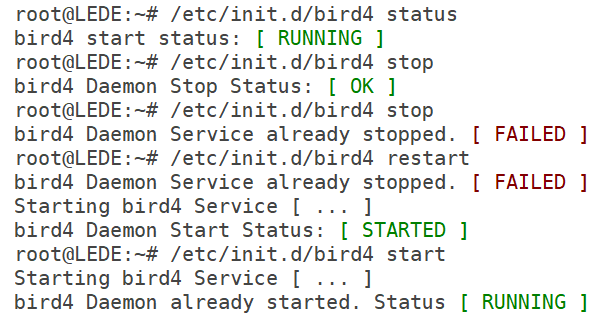
\includegraphics[width=0.7\textwidth]{images/initdterminal}
    \caption{Service management for Terminal.}
    \label{fig:initdt}
\end{figure}

\begin{figure}[ht!]
    \centering
    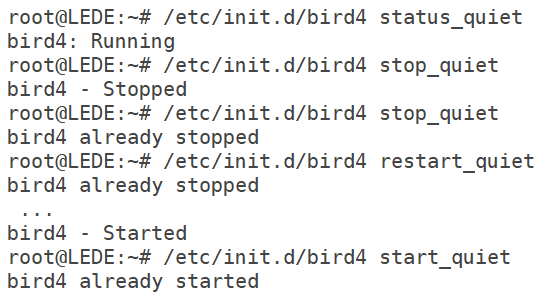
\includegraphics[width=0.7\textwidth]{images/initdui}
    \caption{Service management for Web UI.}
    \label{fig:initdui}
\end{figure}

\subsection{UCI Configuration improvements}
\label{sec:uciimp}
The Unified Configuration Interface (UCI) aims to centralise OpenWrt's settings and it is widely used for almost, if not all, the packages in OpenWrt. UCI allows you to easily, and in a human-readable manner, configure any system following the same scheme, simplifying administration overheads.

However, \textit{bird-uci} Package uses the UCI configuration file in a non-classical manner. Instead of making use of the configuration as it is, the Package only acts as a translator between what the user wants (written in UCI-scheme) and what bird needs to work (c-like configuration file). As stated in section \ref{sec:motivation}, the first version of the package successfully manages Bird, but there have been some API changes since Bird v1.4.3 and the integration is not completed yet:

\begin{itemize}
    \item As part of Bird's v1.4.3 to v1.6.3 API reviewing, some options have required tweaking in order to be compliant to the latest API.
    \item Most of the UCI improvements are tied to LUCI improvements (see section \ref{sec:luciimp}) in order to enhance User eXperience.
    For example, BGP Protocol allows you to execute an action once a number of routes is reached (imported, exported or received). This is shown as a pair of settings in the UI. Previously, each setting was independent, which was a problem as both are optional and hidden for simplicity reasons.
    By adding the extra option, I have been able to tie both options graphically and make them work as expected.
    From /etc/config/bird4:
    \begin{lstlisting}[language=bash,caption={Tied options using UCI (I)}]
config bgp 'bgpAS1'
        option import_trigger '0'
        option export_trigger '0'
        option receive_trigger '0'
        option disabled '0'
        option template 'test123'
        option neighbor_address '192.168.1.100'
        option neighbor_as '1'
\end{lstlisting}

    As shown in the snippet, we have three \texttt{\_trigger '0'} options that state that there is no Limit set in this BGP session. However, if we set one through the UI:
    
\begin{figure}[H]
    \centering
    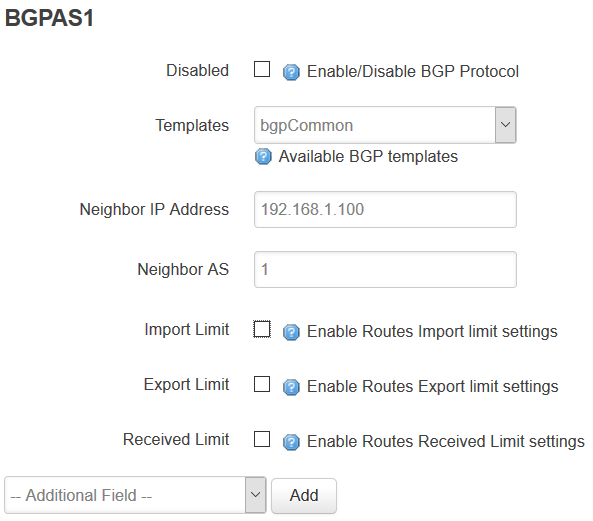
\includegraphics[width=0.8\textwidth]{images/bgp/bgptrigger1}
    \caption{Import Limit Trigger not selected.}
    \label{fig:uitiedn}
\end{figure}

\begin{figure}[H]
    \centering
    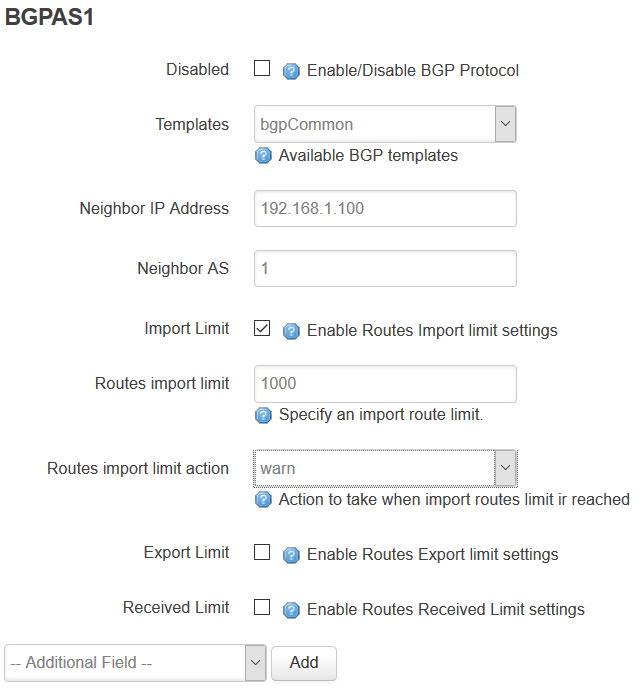
\includegraphics[width=0.8\textwidth]{images/bgp/bgptrigger2}
    \caption{Import Limit Trigger selected.}
    \label{fig:uitiedy}
\end{figure}

As shown in both figures \ref{fig:uitiedn} and \ref{fig:uitiedy} LUCI brings both options together, making it clear to the administrator that these settings must be filled. The UCI result for \ref{fig:uitiedy} is the following:

\begin{lstlisting}[language=bash,caption={Tied options using UCI (II)}]
config bgp 'bgpAS1'
        option import_limit_action 'warn'
        option export_trigger '0'
        option receive_trigger '0'
        option disabled '0'
        option template 'bgpCommon'
        option neighbor_address '192.168.1.100'
        option neighbor_as '1'
        option import_trigger '1'
        option import_limit '1000'
\end{lstlisting}

This tying improvement has been done in the web UI's and not in UCI translation time because, as can be seen in the following code snippet, it is easier to let LUCI configuration management process to add/remove those attributes automatically on settings save time, than doing some hand-made if statements.

In the following LUA snippet, LUCI creates a UI Flag option (our trigger) which is mandatory (\texttt{optional = false}). The other two options (\texttt{limit} and \texttt{limit\_action}) are both optional and dependant on the value of our flag (\texttt{depends({import\_trigger = "1"})}.

\begin{lstlisting}[language=lua, caption={LUCI tied options implementation.}]
[...]
import_trigger = sect_templates:option(Flag, "import_trigger", "Import       Limit", "Enable Routes Import limit settings")
import_trigger.default = 0
import_trigger.rmempty = false
import_trigger.optional = false

import_limit = sect_templates:option(Value, "import_limit", "Routes import   limit", "Specify an import route limit.")
import_limit:depends({import_trigger = "1"})
import_limit.rmempty = true

import_limit_action = sect_templates:option(ListValue,                       "import_limit_action", "Routes import limit action", "Action to take when    import routes limit ir reached")
import_limit_action:depends({import_trigger = "1"})
import_limit_action:value("warn")
import_limit_action:value("block")
import_limit_action:value("disable")
import_limit_action:value("restart")
import_limit_action.default = "warn"
import_limit_action.rmempty = true
[...]
\end{lstlisting}
\end{itemize}

\newpage

\subsection{LUCI UI improvements}
\label{sec:luciimp}
Following previous section's UCI/LUCI example \ref{sec:uciimp}, there have been other UI improvements coupled with changes in the UCI implementation. The following subsections will cover each UI Page to summarise its role and which changes have been done to it. Nevertheless, the last subsection will explain the number of challenges faced during project's development. More detailed images of each page are located in the Appendix \ref{app:ch:extrap}. The ones shown here are for reference.

\subsubsection{Status Page}
New Page allowing an administrator to manage Bird Service. This page shows 3 buttons tied with the init.d functions explained in section \ref{sec:initd} figure \ref{fig:initdui}.


The contents of this page are:
\begin{itemize}
    \item Three buttons to trigger the service management: Start, Stop and Restart in Quiet mode.
    \item Dynamic Text Box showing Bird service's status. This text will be updated if any service update through the buttons is triggered.
\end{itemize}

\begin{figure}[H]
    \centering
    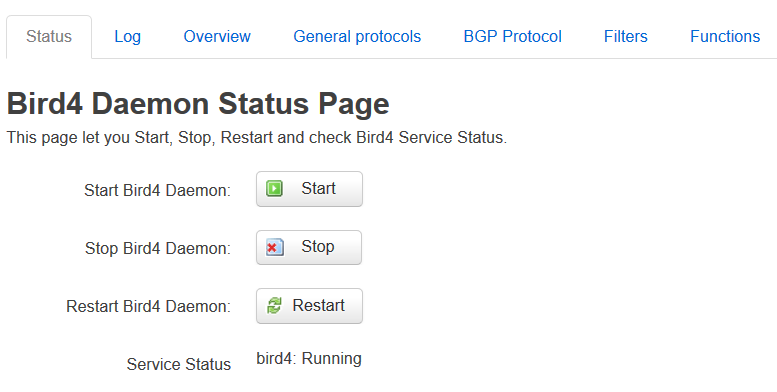
\includegraphics[width=0.8\textwidth]{images/bird0.3/status}
    \caption{Status Page}
    \label{fig:statusp}
\end{figure}

Although contents of this page are simple and straightforward, the result shown in figure \ref{fig:statusp} is not the desired one. The initial idea was to use a single button for starting and stopping the service, and none for restart. Moreover, the button would be automatically switched between states showing, when started, service's PID. In Appendix \ref{app:ch:extrap} you can see the expected behaviour in the implementation of Privoxy's OpenWrt Package.

The reason behind not doing it is that this simple change would require to change from using LUCI's CBI (Lua) to LUCI2 (JavaScript). Lua's implementation allows you to trigger a number of actions according to a specific element state, if an action (e.g. button clicked) is triggered or during page's rendering. However, Bird's startup can take few seconds and LUCI has no granular control or a polling mechanism on rendering time to allow this behaviour. To do so, it would be required to force the page to wait (manual OS \texttt{sleep} command) which would block page's loading and leave it in an incorrect state depending on Bird's time to start.

Nevertheless, I did do a test implementation (with and without a \texttt{sleep} OS call) and, because of the way CBIs work, the button action and rendering action were somehow triggering service calls multiple times, starting and stopping the service in an random way and not refreshing the contents correctly, hence showing wrong status and PIDs.

\subsubsection{Log Page}
\label{sub:sub:logp}
New Page showing contents in Bird's configured Log file. This page is automatically refreshed \textit{each second} with the following information:

\begin{itemize}
    \item Name of the Log file. For reference and easier administration.
    \item Size of the Log file. Critical information in Bird configurations where Debug information is also enabled. Log file can grow really fast if there are more peers sharing information or if the debug mode is set to log most, or all, the possible events in the system.
    If the Log file fills the partition where it is located, Bird will automatically shutdown and prevent any start up attempt until this is resolved. 
\end{itemize}

\begin{figure}[H]
    \centering
    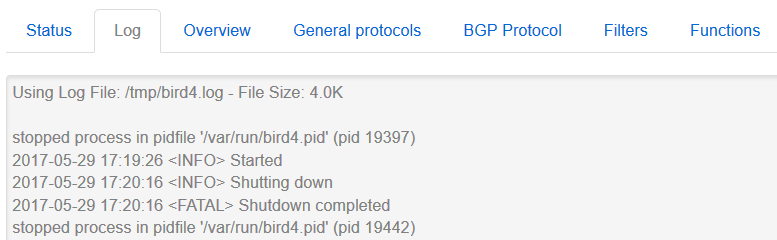
\includegraphics[width=\textwidth]{images/bird0.3/log}
    \caption{Log Page: service restart example}
    \label{fig:statusp}
\end{figure}

This page has been implemented using mixed capabilities from LUCI and LUCI2. Because of the requirement to show a rolling Log page with a reasonably regular auto-refresh process, it was necessary to use JavaScript's XHR capabilities embedded in the HTML page itself together with Lua code to read the file and send the text as a PlainText HTML response (object).

Because of the lack of documentation in this area, I spent weeks investigating it by my own using the available package sources in OpenWrt's repositories. However, because what the other packages usually do is to use XHR polls as a communication broker method (e.g. get a specific data from a specific UCI file, apply some filtering/transformation if the data is not in the desired state and, finally, populate specific UI fields available in the HTML page) it was not clear what exactly I had to do as I only needed to: read last 30 lines of a file (Bird's Log File) and populate the Text View (Plain text data).

Finally, after spending some days trying to contact experienced LEDE/ OpenWrt developers using community's contact channels, I could have few conversations with one of the main contributors of LEDE, OpenWrt and also main author of LUCI/LUCI2 \texttt{jow-}\footnote{Jo-Philip Wich: LEDE-Project and OpenWrt core developer. \href{https://github.com/jow-}{Github Profile}.}, who gave me some hints, examples of LUCI2 pages and also helped me debugging some issues I had during the development that allowed me to finish both Log and Filters/Functions pages.\\

\textbf{Log File Source key highlights:}
\\
Only execute the polling function if \textit{refresh} is passed as parameter.
\begin{lstlisting}[language=lua]
if luci.http.formvalue("refresh") then
\end{lstlisting}

Send the outputs back as plain text.
\begin{lstlisting}[language=lua]
luci.http.prepare_content("text/plain")
\end{lstlisting}

Get the last 30 lines of the file \texttt{log\_file}
\begin{lstlisting}[language=lua]
lf = sys.exec("tail -n30 " .. log_file):gsub("\r\n?", "\n")
\end{lstlisting}

Send, as HTTPResponse object, the quoted message.
\begin{lstlisting}[language=lua]
luci.http.write("Using Log File: " .. log_file .. " - File Size: " .. log_size .. "\n" .. lf)
\end{lstlisting}



\subsubsection{Overview Page}
The Overview Page shows base Bird Service settings:

\begin{itemize}
    \item File used to store the UCI translated Bird.conf file.
    \item Definition of any Routing Table that will be used in the Protocols.
    \item Router's ID (some protocols can overwrite it for their own purposes)
    \item Debug and Log settings and where to store them.
    This option is currently configured to use a single file for logging. However, Bird allows to set any number of different instances with any set of options. Although this would be the desired state, given the resources of most of LEDE/OpenWrt's nodes, the log partition gets filled fast enough with a single file. It is important to know that if the Log Partition is filled and Bird is unable to access it, Bird service will be stopped and blocked until the issue is solved.
\end{itemize}

\begin{figure}[H]
    \centering
    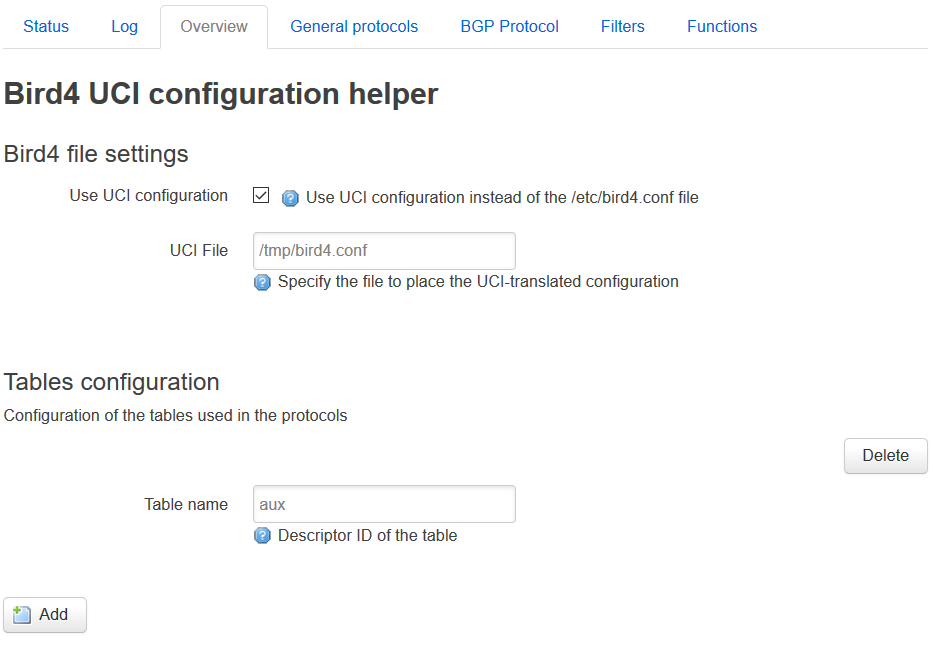
\includegraphics[width=\textwidth]{images/bird0.3/overview}
    \caption{Overview Page}
    \label{fig:overview}
\end{figure}

\textbf{Changes and Improvements:}
This section has not been severely modified. The only big change has been the Log\&Debug settings, because there were some issues using \textit{All} together with other options. By definition, \textit{All} implicitly includes the other options and should not be passed to the configuration.

\subsubsection{General Protocols Page}
The General Protocols Page shows the configuration of some of the Bird support protocols described in section \ref{sub:sub:supproto}.

\begin{itemize}
    \item Kernel Protocol (1 mandatory as base Routing Table talking to the OS. Any extra kernel protocol is optional).
    \item Device Protocol: optional.
    \item Pipe Protocol: optional.
    \item Direct Protocol: optional.
    \item Static Protocol: optional.
    \item Routes: Routes are just the representation of entries in a Static Protocol. These are optional and tied to a single Static Protocol.
\end{itemize}

\begin{figure}[H]
    \centering
    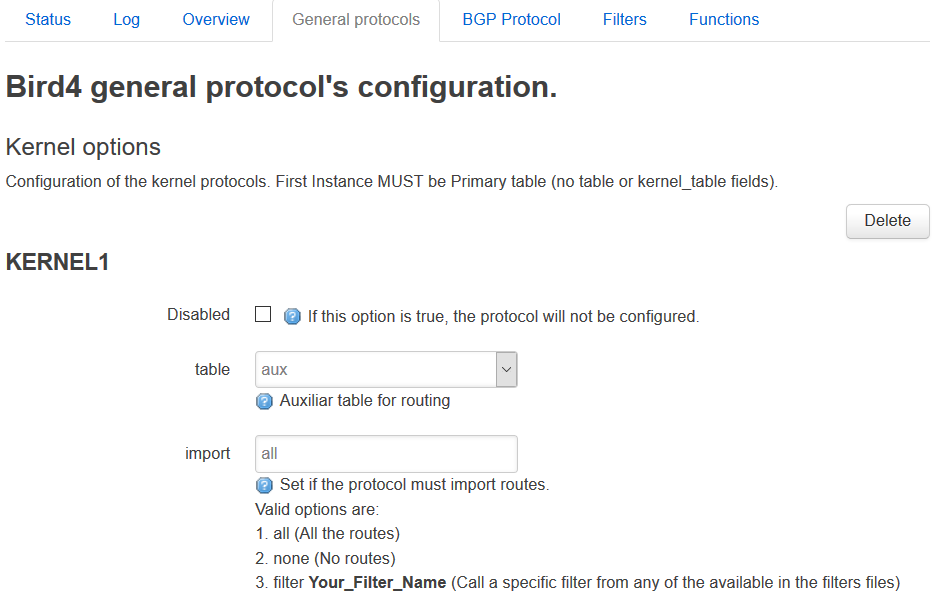
\includegraphics[width=\textwidth]{images/bird0.3/general}
    \caption{General Protocols Page}
    \label{fig:generalp}
\end{figure}

\textbf{Changes and Improvements:}
The main change in this page has been the recovery of both PIPE and Direct Protocols, disabled during the original Project because they were not relevant (there was no coexistence of protocols in Bird). 
These two protocols are now required as they allow to communicate routing tables (PIPE) and to mark the routes as device ones on specific \textit{local} interfaces (DEVICE) to feed the kernel table.

\subsubsection{BGP Protocol Page}
The BGP Protocol Page is the most important for this project as it allows us to configure the main protocol used in Guifi.net. Together with OSPF, BGP is the most complex protocol to configure (and translate) on Bird. With a big number of different \textit{options} as well as another big number of \textit{attributes} to configure, the automation of this protocol has been the main goal of this Package.

\begin{itemize}
    \item BGP Templates: allow to set a number of common options repeated among a number of  different BGP Sessions. Their use simplifies configuration's maintainability as well as improves readability of the file. Templates are optional and you can configure as many as required.
    \item BGP Instances: Instances are the definition of each BGP session to be created. They can feed from Templates or set all the options manually. Instance options will always prevail over template ones. Instances are optional and you can configure as many as required.
\end{itemize}

\begin{figure}[H]
    \centering
    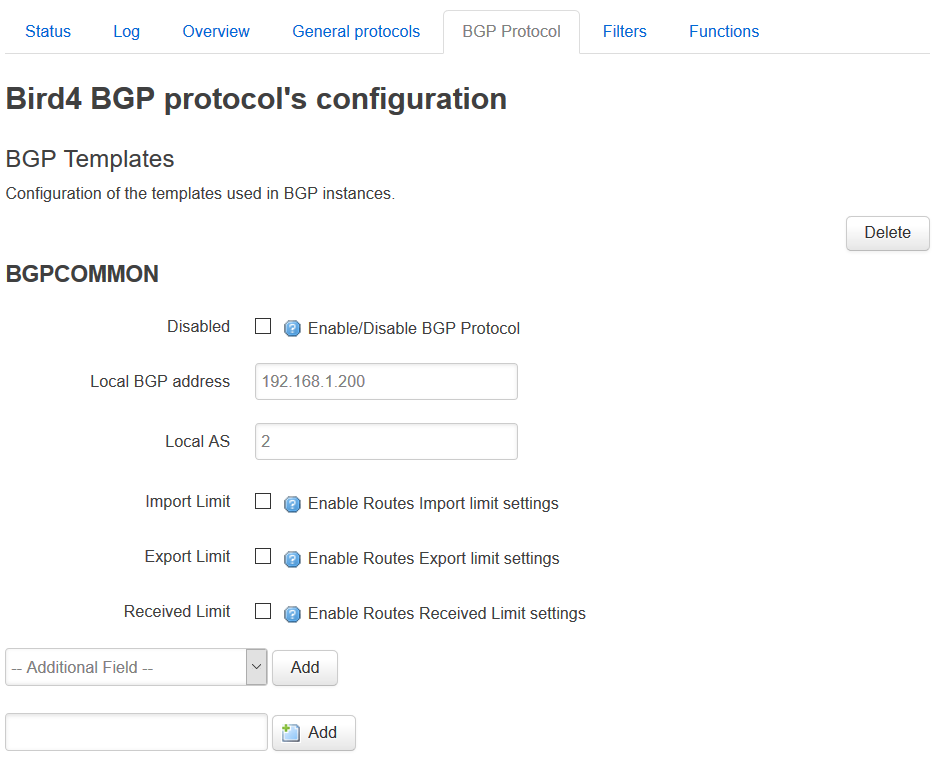
\includegraphics[width=\textwidth]{images/bird0.3/bgp}
    \caption{BGP Protocol Page}
    \label{fig:bgpp}
\end{figure}

\textbf{Changes and Improvements:}
BGP Templates and Instances options have been re-sorted in order to follow a logical order when configuring them. Moreover, all the shown options have been reviewed and re-targeted as optional or mandatory and also, as explained in previous section \ref{sec:uciimp}, some of the options required to configure route sharing limits were not displayed together, which was prone to misconfiguration.

\subsubsection{Filters \& Functions Page}
Two new Pages empowering Filters\&Functions file edition without requiring terminal-based processes. This feature is one of this project's main goals because it completely removes the need for administrators to go to command line, which is a barrier for some non-expert administrators. The page's composition is the following (for both functions and filters):

\begin{itemize}
    \item Disclaimer: informative message about how to rename new files and how to visualise them after creation.
    \item Recognised files dropdown menu: List of the files detected in the correct folder and available for administrators to use. Supported folders are:
    \begin{itemize}
        \item Filters: \texttt{/etc/bird\{4|6\}/filters/*}
        \item Functions: \texttt{/etc/bird\{4|6\}/functions/*}
    \end{itemize}
    \item Load Button: This button will select the file shown in the Text Area and populate the \textit{read-only} Text Box stating which file is actually being edited. Internally, this button will set a Lock variable in the filesystem containing target file name, in order to prevent editing files.
    \item Editing File read-only Text Box: This read-only field is populated with the contents selected in the dropdown menu when the \textit{Load} Button is clicked. Unless this field is populated with a full path to a file, any contents in the TextArea will dropped (\texttt{Submit} button will just refresh the contents of the page).
    \item Text Area Box: This editable 30 lines field will be populated with the contents of the file Loaded (or empty if it is a new file). Any contents in this field will be stored in the selected file, or dropped otherwise.
    \item Submit Button: This button will trigger the save mechanism. If a file has been correctly loaded, it will store the contents in the Text Area to the target file. Protocol's configuration can be stored before applying it by clicking the \textit{Save} button instead of the \textit{Save \& Apply} on. However, this process uses direct system calls and is not reversible, hence it is named \textit{Submit}.
\end{itemize}

\begin{figure}[H]
    \centering
    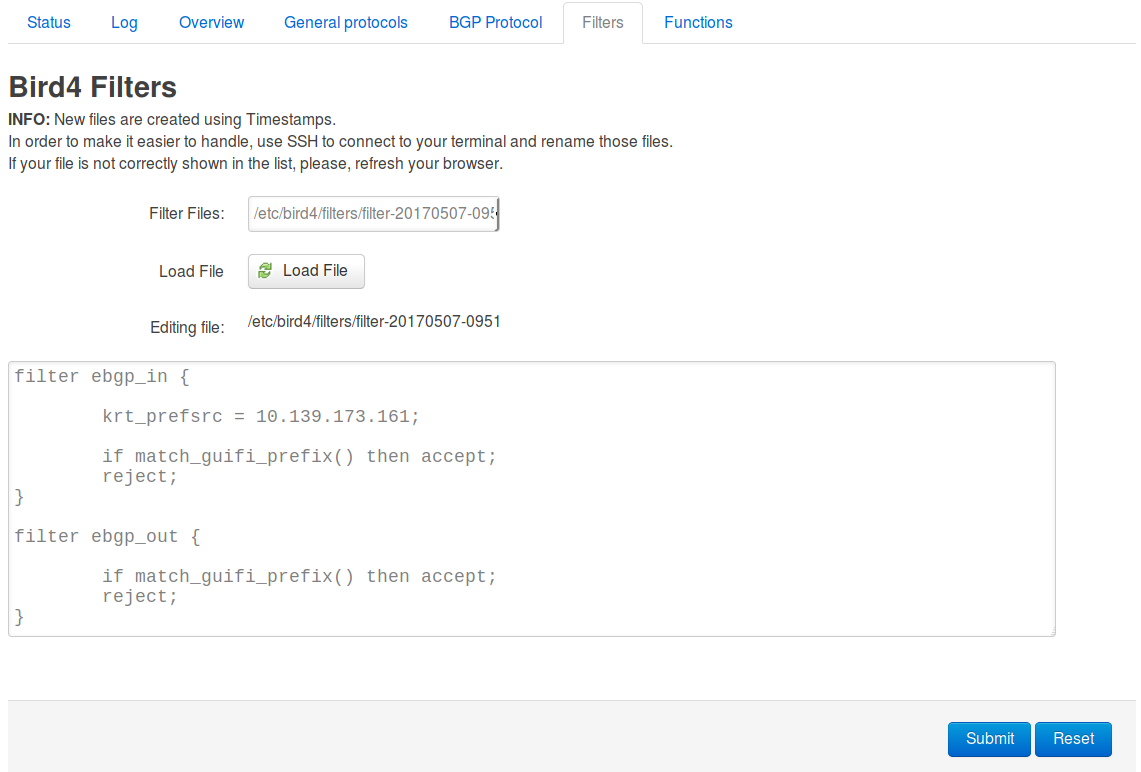
\includegraphics[width=\textwidth]{images/bird0.3/filters}
    \caption{Filters Page}
    \label{fig:filtersp}
\end{figure}

\begin{figure}[H]
    \centering
    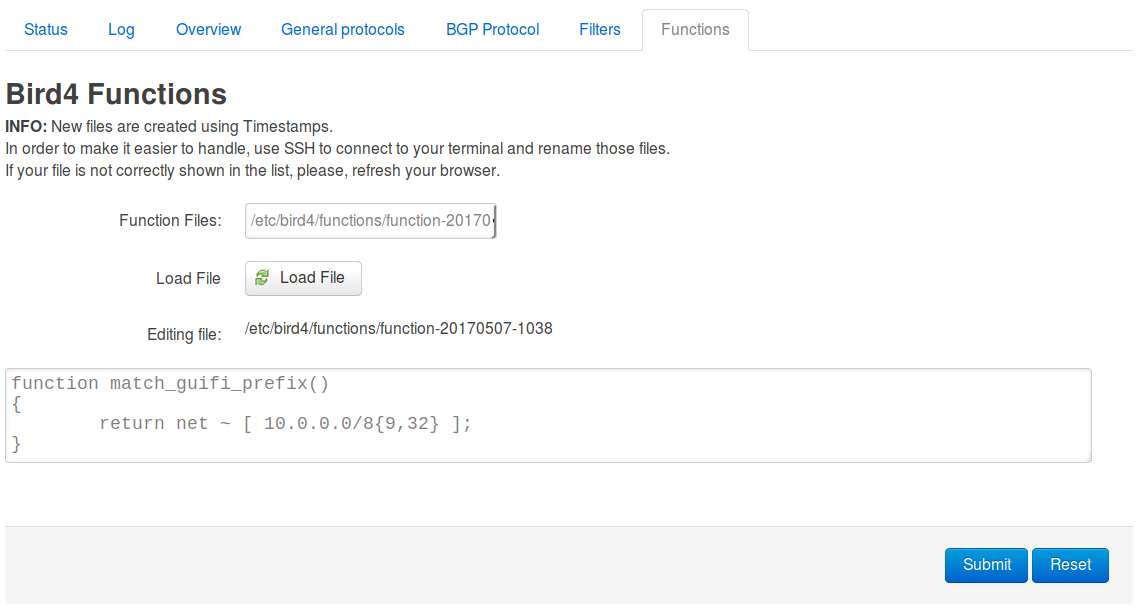
\includegraphics[width=\textwidth]{images/bird0.3/functions}
    \caption{Functions Page}
    \label{fig:functionsp}
\end{figure}

These two pages have been implemented using LUCI capabilities only (Lua Model) plus a simple HTML template, with some Lua embedded to inject text and properties, in order to enhance the Text Area: set to 30 lines, enlarge text's size and make use of \texttt{Courier New} font in order to make it more \textit{console-alike} highlighting that it is code and not plain text:

\begin{lstlisting}[language=javascript,caption={Enhanced Edit Text Box Template}]
<%+cbi/valueheader%>
    <textarea class="cbi-input-textarea" <% if not self.size then %>         style="width: 100%; font: normal 11pt 'Courier New'"<% else %> cols="<%=self.size%>"<% end %> data-update="change"<%= attr("name", cbid) .. attr("id",    cbid) .. ifattr(self.rows, "rows") .. ifattr(self.wrap, "wrap")  ..          ifattr(self.readonly, "readonly") %>>
    <%-=pcdata(self:cfgvalue(section))-%>
    </textarea>
<%+cbi/valuefooter%>
\end{lstlisting}

\begin{itemize}
    \item \texttt{<\%+cbi/valueheader\%>} and \texttt{<\%+cbi/valuefooter\%>}: Lua snippets acting as delimiters for top and bottom cbi's contents.
    \item \texttt{<\%[...]\%>}: Lua code injection.
    \item \texttt{<\%=[...]\%>} Lua variable injection.
\end{itemize}

\textbf{Caveats}\\
The biggest challenge has been to be able to select different files to store our filters and functions. This Page has required a couple of weeks of development because of its functionality, the already mentioned file selection flexibility and what is required from the Text Area is not something easy to do with current LUCI documentation.

In the same way as the Log Page \ref{sub:sub:logp}, current documentation refers to the most common uses but pages where no UCI configuration is involved are just briefly mentioned. Some of the challenges found are:
\begin{itemize}
    \item \texttt{SimpleForm} Page format is required due the lack of UCI settings to modify. However, the documentation explaining which is SimpleForm's API, differences between this solution and \texttt{Map}\footnote{Map is LUCI's alternative format page to define UI by \textit{mapping} fields into UCI properties} or possibilities using SimpleForm are not detailed enough.
    \item Local variables are not reliable. Because pages can be re-rendered depending on the event triggered, your stored variables could be overwritten with new values by these rendering functions.
    An example of this issue was my attempt use the Read-only field to store the path. Because \texttt{cfgvalue} (render) function is triggered several times in an uncontrolled manner (we have no control of it) your variable may have been overwritten several times. Therefore, if you switch the selected file, you were storing your data in the wrong file.
    \item UI values can only be gathered or saved during specific events (e.g. on render or save functions).
    \item Unable to refresh the file list on a render function. It has bee required to do it as part of Page's creation, therefore, needing to refresh the page to update the file list. This is \textit{annoying} if you have created a new file, because it may not be listed until you refresh the page.
    This has been documented as a known issue and will be resolved by using LUCI2 in a future release. 
    \item Trying to use nested events usually cause data misconfiguration.
    An example of that was my first attempt to use the Load File Button to lock the target file. Current process to edit files is: 
    \begin{itemize}
        \item Select a file
        \item Press Load Button
        \item The file is Loaded (write Lua function): filename in the readonly field and contents in the TextArea.
        \item Edit File contents
        \item Press Submit (write Lua function)
    \end{itemize}
    Because the Submit button also triggers a write Lua function, it was, somehow, also activating Load Button's one. This was a big issue if, before saving the file, the administrator selects a different file from the dropdown menu.
    This issue was finally solved by adding an extra level of complexity on both write Lua functions as well as storing our target path in a file in the system (\texttt{/etc/bird\{4|6\}/filter\_lock} and \texttt{/etc/bird\{4|6\}/ffunction\_lock}).
\end{itemize}



\subsection{Align documentation and upgrade to Markdown}
Documentation has been one of the biggest disappointments while working with LUCI/LUCI2. To use a project or a technology and find that there is not enough detail, if any, about what you can do and how, is really disappointing and causes frustration while trying to figure it out. Therefore, I have put a lot of efforts on updating all the documentation available in the Package, as well as added an extra repository with other data that supports it, without bloating it (this Package will be Pulled to the official repository, so it is desirable to have the minimum contents in this one, and everything else linked). Moreover, because the old documentation was plain text, it was unpleasant to read. In order to facilitate Package's configuration and daily usage, I have upgraded old documents to \Gls{markd}.

The main documentation is now separated between:
\begin{itemize}
    \item UCI: UCI definition and examples and any terminal-based function or command required to use the Package without UI.
    \item LUCI: Web UI Pages' composition, field description, default values and any known issue.
    \item README.md: Development notes about how to build and enhance the Package and known issues on current Package version.
    \item Changelog.md: Exhaustive list of enhancements added as part of this project (v0.3)
    \item COPYING.md: Markdown version of GPLv3.0
    \item AUTHORS.md: List of the contributors.
\end{itemize}

Documentation repository with extra information:
\begin{itemize}
    \item Repository-Contents.md: This file includes the tree structure of Packages repository as well as a description of what each file is.
    \item Manual-Procedures.md: List of manual procedures that have not been automated in this Package's version and may require an administrator to do them on command line.
    Currently the use of secondary Routing Tables with custom table IDs has to be done following the procedure shown.
    \item TODO.md: Unsorted and non-prioritised list of tasks pending for future releases.
\end{itemize}

\section{Bird Daemon uBus integration investigation}
uBus theoretical investigation is driven by the need of continuously monitor the status of our protocols and the critical historical data that it could bring any administrator managing any size and complexity networks. Current Bird's implementation provides a low consumption and powerful routing solution but its monitoring capabilities lay in a \acrshort{cli} mimicking other well-known plain text-based tools as Quagga, Cisco or Mikrotik's Consoles.

OpenWrt/LEDE's Bird plain-text CLI tools are \texttt{birdc\{4|6\}} and \texttt{birdcl\{4|6\}}. Birdcl is the lightweight version of birdc. It does not support some commands (e.g. service management) or command history. Both tools provide the administrators an API \cite{birdcapi} in order to manage the live system and gather information from it using UNIX Standard domain sockets (\texttt{bird.ctl}). As already mentioned, this CLI provides human readable plain-text information on specific queries, thus most of its outputs are not suitable or automatizable for scripting. Some example of Birdc's outputs are:

\begin{lstlisting}[language=bash, caption={Birdc Console mode.}]
root@LEDE-MXN1:/etc/config# birdc4
BIRD 1.6.3 ready.
bird> show status
BIRD 1.6.3
Router ID is 10.139.173.161
Current server time is 2017-06-03 19:06:59
Last reboot on 2017-06-03 00:54:23
Last reconfiguration on 2017-06-03 00:54:23
Daemon is up and running
bird> show protocols
name     proto    table    state  since       info
kernel1  Kernel   aux      up     00:54:22
static1  Static   aux      up     00:54:22
device1  Device   master   up     00:54:22
BCNRamblaPobleNou BGP      aux      up     00:54:27    Established
UOCBGPMesh BGP      aux      down   00:54:22
bird> exit
root@LEDE-MXN1:/etc/config#
\end{lstlisting}

This example shows two output examples of Bird CLI working in Console mode. The administrator enters into a Bird-protected-mode in order to visualize the required information. The tool also includes a helper function (command: \texttt{?}) according to the specific command being visualised:\\

\begin{lstlisting}[language=bash, caption={Help on Birdc Console mode.}]
bird> ?
add roa ...                                    Add ROA record
configure ...                                  Reload configuration
debug ...                                      Control protocol debugging via BIRD logs
delete roa ...                                 Delete ROA record
disable <protocol> | "<pattern>" | all         Disable protocol
down                                           Shut the daemon down
dump ...                                       Dump debugging information
echo ...                                       Control echoing of log messages
enable <protocol> | "<pattern>" | all          Enable protocol
eval <expr>                                    Evaluate an expression
exit                                           Exit the client
flush roa [table <name>]                       Removes all dynamic ROA records
help                                           Description of the help system
mrtdump ...                                    Control protocol debugging via MRTdump files
quit                                           Quit the client
reload <protocol> | "<pattern>" | all          Reload protocol
restart <protocol> | "<pattern>" | all         Restart protocol
restrict                                       Restrict current CLI session to safe commands
show ...                                       Show status information
bird>
\end{lstlisting}

\begin{lstlisting}[language=bash, caption={Help on \texttt{show} level of Birdc Console mode.}]
bird> show ?
show bfd ...                                   Show information about BFD protocol
show interfaces                                Show network interfaces
show memory                                    Show memory usage
show ospf ...                                  Show information about OSPF protocol
show protocols [<protocol> | "<pattern>"]      Show routing protocols
show rip ...                                   Show information about RIP protocol
show roa ...                                   Show ROA table
show route ...                                 Show routing table
show static [<name>]                           Show details of static protocol
show status                                    Show router status
show symbols ...                               Show all known symbolic names
bird>
\end{lstlisting}

Finally, the following code snippet shows our target information: BGP Session live data.

\begin{lstlisting}[language=bash, caption={Birdc Simple \texttt{Show Protocols all}. Truncated to show BGP.}]
root@LEDE-MXN1:/etc/config# birdc4 show protocols all
BIRD 1.6.3 ready.
name     proto    table    state  since       info
BCNRamblaPobleNou BGP      aux      up     00:54:28    Established
  Preference:     100
  Input filter:   ebgp_in
  Output filter:  ebgp_out
  Routes:         3023 imported, 0 exported, 3023 preferred
  Route change stats:     received   rejected   filtered    ignored   accepted
    Import updates:         108200          0          0         13     108187
    Import withdraws:        25629          0        ---          6      25623
    Export updates:         108187     108187          0        ---          0
    Export withdraws:        25623        ---        ---        ---          0
  BGP state:          Established
    Neighbor address: 172.25.35.25
    Neighbor AS:      59361
    Neighbor ID:      10.90.224.65
    Neighbor caps:    refresh AS4
    Session:          external AS4
    Source address:   172.25.35.26
    Hold timer:       164/180
    Keepalive timer:  28/60
\end{lstlisting}

As shown in the snippet above, we can query Bird to get base BGP information: name, session status, path preference, neighbour's ID, etc. Or live data as Keepalive time left or number of routes imported, exported, blocked by our filters, etc. This information would be valuable for administrators if it was shown in the UI as a chart or rolling text field, working both as live status checker and also as a health screener.

Understanding that our main goal is to, somehow, integrate monitoring capabilities into the Package, the next step is to see which tools would support us doing it.

\subsection{LUCI2 new architecture: WebUI-uBus-RPCd-Service}
\label{sub:luci2arch}
LUCI2 introductory information is available in section \ref{sub:sub:luci2}, see it for reference of the acronyms.

LUCI2 main components are: 

\begin{itemize}
    \item Client-Side Browser: HTML/CSS/JS provided by service (e.g. luci-app-bird\{4|6\}) is executed on client's side.
    \item uBus Service: Client-Server-based query broker to communicate different system services.
    \item uHTTPd Server: \textit{Server-side} HTTP server to satisfy queries.
    \item RPC Daemon: HTTP backend server acting as a query broker for packages not integrated with uBus service but providing an API to use it.
\end{itemize}


\subsubsection{Example overview}

Using Bird4, luci-app-bird4 and a fictional \textit{RPC-uBus Bird4 Service} as an example, this process' architecture is the following:

\begin{figure}[H]
    \centering
    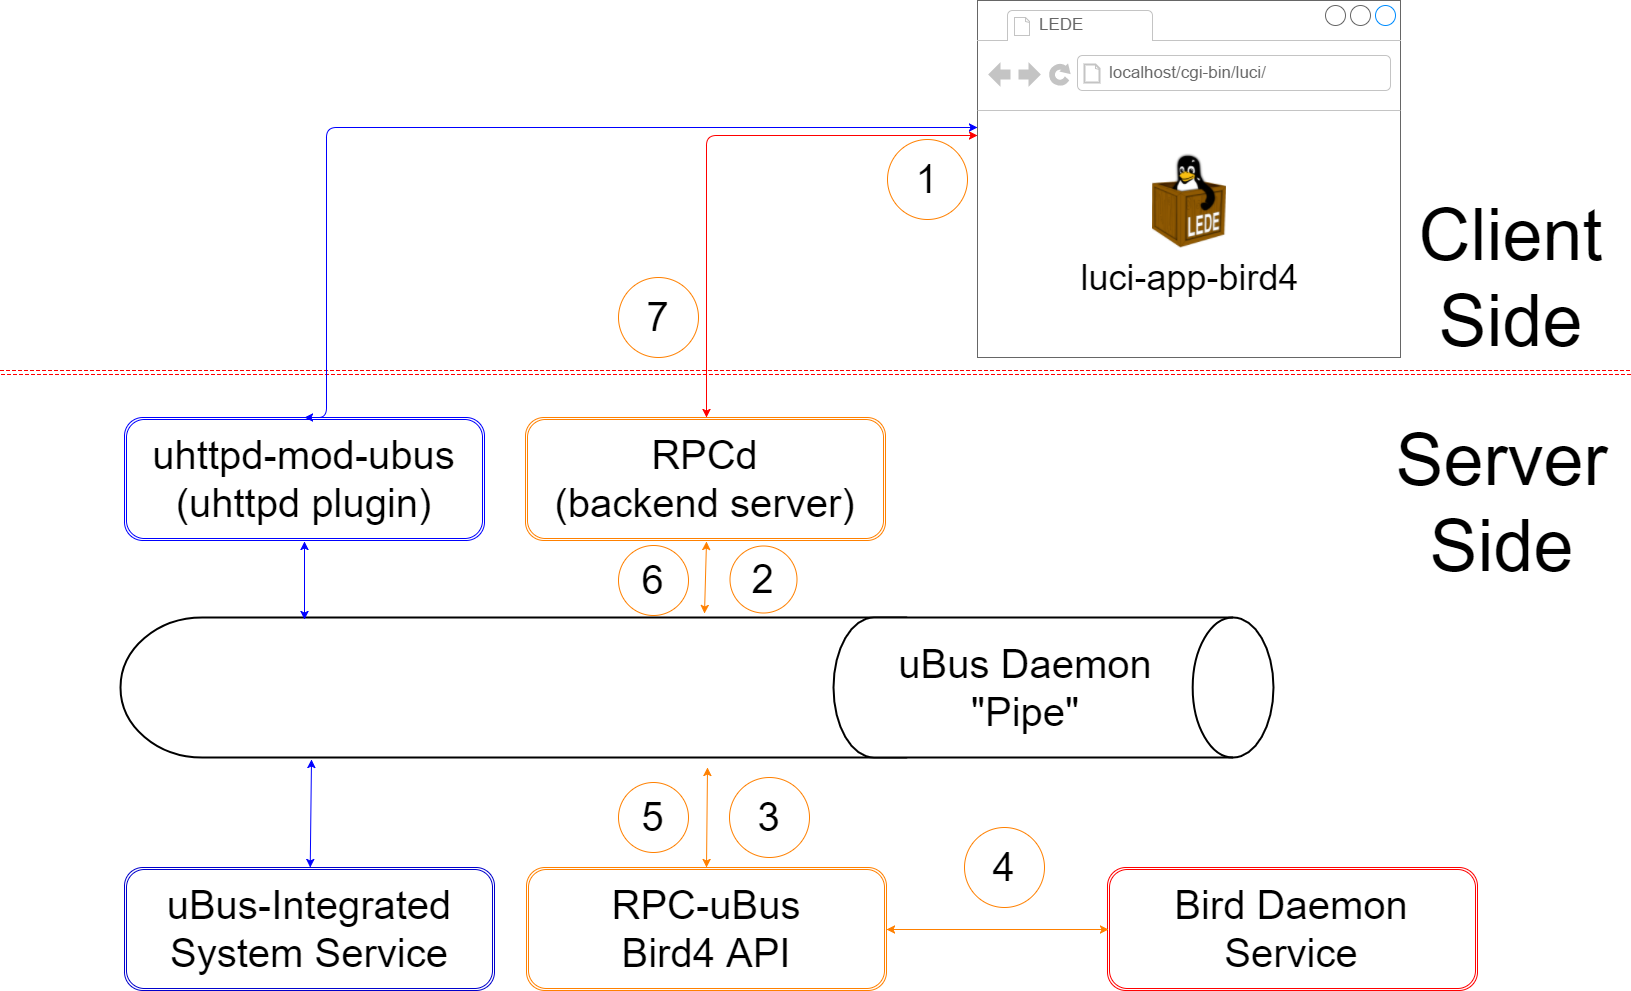
\includegraphics[width=\textwidth]{images/luci2/luci2d}
    \caption{LUCI2 Communication architecture for Bird4 Service}
    \label{fig:luci2arch}
\end{figure}

Taking in consideration that Bird has no integration with uBus, we need to connect to it through an RPCd service. The steps followed for a Client to interact with Bird Service are shown in figure \ref{fig:functionsp}:
\begin{enumerate}
    \item Client's browser wants to query Bird service to populate a number of fields the UI (luci-app-bird4). These queries are done using JavaScript using RPCd's API.
    \item RPCd backend server passes Bird's UI query to uBus, who will check if Bird has an API registered in  its namespace.
    \item If uBus finds the given API, it checks the specific call sent and it is executed.
    \item Bird4's API executes shell script commands to directly query Bird4 and returns any outputs generated.
    \item The API will need to handle Bird's outputs and to encapsulate them into JSON objects. After doing that, any generated output is sent back to uBus.
    \item uBus sends any object received to the RPCd server.
    \item RPCd Server sends this object back to the client and it refreshes any targeted component with this new data.
\end{enumerate}

\subsubsection{Server-side's implementation details}
Following the bullets above, the first thing required is to create our \textit{Shell} API under the folder \texttt{/usr/libexec/rpcd} for uBus to be able to add it. This API needs to provide its own description (\texttt{list}) and functions (\texttt{call}) required to communicate your service through JSON objects with the Client. This example shows a Bird service management implementation using four RPC calls (see figure \ref{fig:functionsp}: step number 3).

\begin{lstlisting}[language=bash,label={lst:rpcbird},caption={RPCd Bird4 Service Management.}]
#!/bin/sh

case "$1" in
    list)
        echo '{ "status": { }, "start":{ }, "stop":{ } }'
    ;;
    call)
        case "$2" in
            status)
                status=$(/etc/init.d/bird4 status_quiet)
                echo "{ \"status\" : \"$status\" }"
            ;;
            start)
                start=$(/etc/init.d/bird4 start_quiet)
                echo "{ \"start\" : \"$start\" }"
            ;;
            stop)
                stop=$(/etc/init.d/bird4 stop_quiet)
                echo "{ \"stop\" : \"$stop\" }"
            ;;
        esac
    ;;
esac
\end{lstlisting}

On a new system, where no other services have been registered on RPCd, if we check what is registered on uBus, we will see only system services:

\begin{figure}[H]
    \centering
    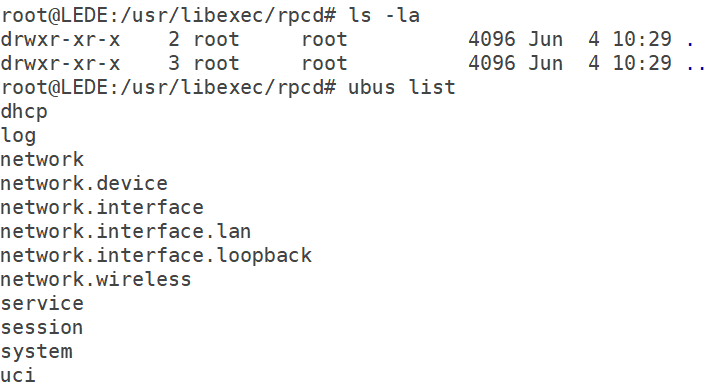
\includegraphics[width=\textwidth]{images/luci2/step1}
    \caption{uBus registered services (I)}
    \label{fig:ubusrs1}
\end{figure}

We can see in the figure that no other services are providing an API using RPCd folder (it is empty) and we can only find services like network, UCI or system itself providing uBus integration.

After adding our code shown in the snippet \ref{lst:rpcbird} in RPCd's folder and restarting RPCd service, we can now start querying it:

\begin{figure}[H]
    \centering
    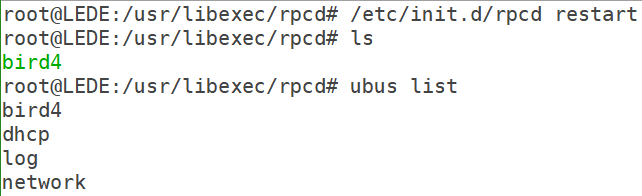
\includegraphics[width=\textwidth]{images/luci2/step2}
    \caption{uBus registered services (II)}
    \label{fig:ubusrs2}
\end{figure}

The truncated output shows that uBus is now able to call bird functions. If we query uBus for specific and verbose (\texttt{-v}) information about the provided API this would be the output:

\begin{figure}[H]
    \centering
    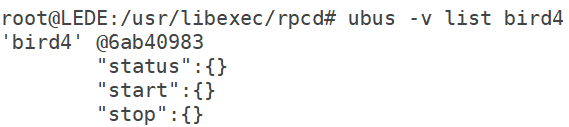
\includegraphics[width=\textwidth]{images/luci2/step3}
    \caption{uBus registered services (III)}
    \label{fig:ubusrs3}
\end{figure}

As show in the figure \ref{fig:ubusrs3}, this Bird RPCd API provides 3 functions requiring no parameters (an example of a parametrized API will be shown as an example for Client-side's example).

Now we can test this API, which is interacting (in an over-simplified manner) with Bird:

\begin{figure}[H]
    \centering
    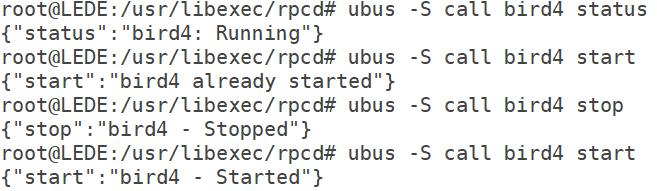
\includegraphics[width=\textwidth]{images/luci2/step4}
    \caption{uBus registered services (IV)}
    \label{fig:ubusrs4}
\end{figure}

As shown in the code snippet \ref{lst:rpcbird}, we are executing \texttt{*\_quiet} functions returning plain text responses from Bird service's management script. This output is wrapped in a JSON object and uBus will send this output back to the Client.

With these steps, we have all the necessary elements to make RPCd communicate from server's side.

\subsubsection{Client-side implementation details}

This client-side example is different from the server-side one and has not been implemented in the development environment. It adds extra complexity in order to be able to tie it with the next subsection \ref{sub:sub:birdex}, which will cover the required changes in Bird itself in order to support LUCI2.

Code snippet \ref{lst:luci2rpc} could be part of a future version of luci-app-bird\{4|6\} or a new package adding this functionality separately as a plugin (e.g. \texttt{bird-mod-ubus}). This example explores the possibility of a future BGP monitoring page (or section in BGP Protocols Page) giving administrators live information about their sessions.

\begin{lstlisting}[language=javascript,label={lst:luci2rpc},caption={RPC Call Script.}]
Luci2().ui.view.extend({
[...]
    getPeers  : Luci2().rpc.declare({
        object: 'bird4',
        method: 'getBGPNeighbour',
        params: '[ "BGPSession" : "' + targetBGPSession + '" ]',
        expect: { BGPNeighbourID: {} }
    }),
[...]
    getNeighbourStatus : function() {
        var targetBGPSession = "BCNPeerToTGN";
        self.getPeers(targetBGPSession).then( function(JSONOutput)
        {
            // Parse any JSON Data received into a pre-defined and sanitised format
            var bgpData = self.parseJSON(JSONOutput);
    
            // Update the UI according to the data received
            self.updateUIData(bgpData);
        });
    },
[...]
    execute: function () {
        [...]
        // Force RPC call to be called each second
        self.repeat(self.getNeighbourStatus, 1000);
        [...]
    }
}
\end{lstlisting} 

This possible JavaScript code defines the API used in order to communicate with the backend server (\texttt{declare}) calling bird4's RPCd and querying the \texttt{getBGPNeighbour} function. This function would, somehow, query \texttt{birdc4} (e.g. \texttt{birdc4 show protocols "BCNPeerToTGN" -json '\{ 'bgpPeerID' : \{ \} \}'}) or any other tool designed for Bird to answer live data queries with JSON-formatted responses instead of human-readable ones.
This snippet follows an oversimplified approach where we only ask Bird for a specific data and we use only a little portion of it (BGP Neighbour AS ID). However, I mention both \texttt{parseJSON} and \texttt{updateUIData} on purpose foreseeing that this RPC function would really return all BGP's data and populate the UI with it in a reasonable time lapse (snippet shows 1 second repetition).

\subsubsection{Bird Service's required changes}
\label{sub:sub:birdex}
Previous sections have explained how we could implement an integration of Bird in uBus presupposing that it is already providing JSON-formatted outputs.
This section focuses on Bird's implementation and which changes would be required to support this new output format.

For this investigation, I have reviewed three possible approaches:

\begin{enumerate}
    \item \textbf{Generate a new OpenWrt package to parse Bird's outputs from human-readable to JSON}:\\
The first approach is to use Bird Remote Control's command outputs in the same human-readable format (see example shown in the snippet \ref{lst:birdchr}). This would require specific parsing functions for each possible output and variation (e.g. while established BGP sessions show detailed route data, non-established ones show no information). This solution would have no impact in Bird's official code as JSON parsing would occur in a separate software.
    
This option is totally dismissed as it adds two levels of complexity by forcing the new package (or functionality) to be parsing messages and being completely coupled with a non-standard and unreliable communication \textit{API}. Therefore, any change in Bird's human-readable outputs or data's structure shown would cause our package to stop working and to require a parser update to conform to the new API. All this process would take some time and could be challenging according to which non-standard part of the output has changed, affecting any users on OpenWrt/LEDE systems.


    \item \textbf{Modify Bird Remote Control's implementation to parse from human-readable to JSON}:\\
This second approach moves the JSON parsing closer to where it is originated. Birdc and Birdcl tools just \texttt{echo}es the data according to the CLI command executed. However, unlike the first approach, because the outputs are parsed on Bird's side, their community and developers would manage any required integration change in order to support the latest version of the Daemon. Hence, any external administrator or developer would be able to rely in a standardised API with JSON-formatted outputs.

This option has also been dismissed because, although the parsing method occurs closer to the data, there is still a parsing method from Bird's human-readable output to JSON. Moreover, any external developer requiring live data would be forced to:

\begin{itemize}
    \item Forced to use or, at least, to install a tool not fit for purpose (CLI).
    \item Use a socket to Bird which is not exclusive to his processes.
    \item Use a socket to Bird which its \textit{private} API could be accessible from the CLI tool.
    \item In order to get some data, it could be required to use CLI-based commands.
\end{itemize}

    \item \textbf{Modify Bird's code to switch from human-readable to JSON outputs}:\\
This third approach moves the problem even further. The solution proposed is to modify Bird's code in order to add extra functions that would, together with the human-readable ones, present protocols' live status in JSON format. This means that we have to review Bird's code in order to find where each output is generated and create an extra function (or add a parameter) to send the data in JSON's format.

This proposal requires a high number of changes in the official solution as well as tests to prove that all generated outputs are RFC compliant \cite{json} and that this changes are not causing performance issues in the Daemon. Following this solution, it could open three new options to solve our current issues:
   \begin{itemize}
        \item Continue using Bird Remote Control but receiving JSON outputs instead of human-readable ones (may require improvements in birdc/birdcl tools).
        This option has some of the 2\textsuperscript{nd} proposal issues.
        \item Create a new bird \textit{semi-official} (while not accepted) utility following the same approach of birdc (UNIX socket to connect to Bird) only being used for monitoring purposes.
        This solution would require its own UNIX socket or to use the same as Bird Remote Control, which could create a conflict.
        \item Create an integration package or specific Bird implementation with uBus Socket. This would be the desired solution as the communication and integration would be complete and Bird could be announced as uBus \textit{compliant} service. Moreover, on the one hand there would be no conflicts with Bird Remote Control but, on the other hand, there could be some performance issues derivatives from this (currently unknown) socket communication implementation.
   \end{itemize}

Finally, as an example of Bird's current output printing implementation, the following snippet shows part of BGP's  information presentation \cite{bgpsn}:

\begin{lstlisting}[language=javascript,label={lst:bgpcode},caption={bgp\_show\_proto\_info function in BGP.c.}]
static void
bgp_show_proto_info(struct proto *P)
{
    struct bgp_proto *p = (struct bgp_proto *) P;
    struct bgp_conn *c = p->conn;

    proto_show_basic_info(P);

    cli_msg(-1006, "  BGP state:          %s", bgp_state_dsc(p));
    cli_msg(-1006, "    Neighbor address: %I%J", p->cf->remote_ip, p->cf->iface);
    cli_msg(-1006, "    Neighbor AS:      %u", p->remote_as);
[...]
}
\end{lstlisting}

This code snippet \ref{lst:bgpcode} shows the first lines of BGP's information, available even if the session fails. The main idea from this snippet is that all the different protocols available in Bird are using C data structures in a non-obscured manner, with some of the almost identical to JSON:\\E.g. \texttt{p->rr\_client ? " route-reflector" : "",}\\Next code snippet shows BGP Connection structure (one of the different BGP structures):

\begin{lstlisting}[language=javascript,label={lst:bgpstruct},caption={Bird's BGP Protocol Session C Structure.}]
struct bgp_conn {
  struct bgp_proto *bgp;
  struct birdsock *sk;
  uint state;				/* State of connection state machine */
  struct timer *connect_retry_timer;
  struct timer *hold_timer;
  struct timer *keepalive_timer;
  struct event *tx_ev;
  int packets_to_send;			/* Bitmap of packet types to be sent */
  int notify_code, notify_subcode, notify_size;
  byte *notify_data;
  u32 advertised_as;			/* Temporary value for AS number received */
  int start_state;			/* protocol start_state snapshot when connection established */
  u8 peer_refresh_support;		/* Peer supports route refresh [RFC2918] */
  u8 peer_as4_support;			/* Peer supports 4B AS numbers [RFC4893] */
  u8 peer_add_path;			/* Peer supports ADD-PATH [RFC7911] */
  u8 peer_enhanced_refresh_support;	/* Peer supports enhanced refresh [RFC7313] */
  u8 peer_gr_aware;
  u8 peer_gr_able;
  u16 peer_gr_time;
  u8 peer_gr_flags;
  u8 peer_gr_aflags;
  u8 peer_ext_messages_support;		/* Peer supports extended message length [draft] */
  unsigned hold_time, keepalive_time;	/* Times calculated from my and neighbor's requirements */
};
\end{lstlisting}

Therefore, we could make use of some available implementations to automate their parsing (e.g. \Gls{jsonc}) and make the integration process much easier and facilitate its maintainability.
\end{enumerate}


\subsubsection{Analysis conclusions}
The conclusion I reached from this theoretical analysis about the feasibility of integrating uBus on Bird is that, although it would require a lot of efforts until we can viably get JSON-formatted live data from Bird, it is possible to achieve it if the third approach I have presented is followed. This approach will require Bird community and developers' support in order to implement it in the official stream and this solution must follow JSON standards. After achieving that, we can start defining how we want current LUCI or LUCI2 implementation's to adopt this new API and how much it can be delivered in an initial phase (from simple auto-refreshed text fields to historical health charts, simulated connectivity maps and other relevant data).

Joining everything together, these requirements would easily  become a feasible future Open Source Software MSc. project. This project's requirements would be: to have network's knowledge or willingness to learn about it; to have some level of C, Shell and JavaScript expertise; to be prepared to agree project's requirements, ideas and approaches with Bird's community and developers; and also patience to deal with the lack of LUCI2, uBus and RPCd documentation in OpenWrt/LEDE, being a bonus if, together with the community, the student helps to fill any knowledge gaps and to feed them back to them.

\newpage